\documentclass[10pt,journal,compsoc]{IEEEtran}

\usepackage{amsmath,amssymb,amsfonts}
\usepackage{booktabs}
\usepackage{graphicx}
\usepackage{url}
\usepackage{hyperref}
\usepackage{cite}
\usepackage{tikz}
\usepackage{pgfplots}
\pgfplotsset{compat=1.18}
\usetikzlibrary{shapes.geometric, arrows, positioning}

\hypersetup{
    colorlinks=true,
    linkcolor=blue!70!black,
    citecolor=blue!70!black,
    urlcolor=blue!70!black
}

\begin{document}

\title{SecretGuard: Autonomous, Privacy-Preserving Secret Interception and Tiered Ambiguity Quarantine for Version Control Systems}

\author{Anuska~Saha%
\thanks{The author is with the Department of Computer Science and Engineering. Email: correspondence@example.org. Code and reproducibility artifacts are available in the project repository.}%
}

\markboth{IEEE Transactions on Software Engineering,~Vol.~XX, No.~X,~October~2026}%
{Saha: SecretGuard: Autonomous Secret Interception and Quarantine}

\maketitle

\begin{abstract}
Accidental leakage of authentication credentials, cryptographic private keys, and application programming interface (API) tokens into public and private software repositories remains a primary attack vector in modern software supply chains. While static application security testing (SAST) tools and pre-commit linters attempt to intercept sensitive strings prior to version control submission, existing solutions present a severe operational dilemma: fast deterministic scanners rely on coarse regular expressions and raw entropy calculations that suffer from prohibitive false-positive rates, whereas emerging cloud-based Large Language Model (LLM) verifiers introduce intolerable commit-time latency, high monetary cost, and the hazard of transmitting proprietary intellectual property to remote endpoints. In this paper, we introduce \textbf{SecretGuard}, an autonomous, privacy-preserving credential interception and quarantine engine tailored for Git pre-commit hooks and local continuous integration pipelines. SecretGuard resolves the speed--precision tension through a three-tier hybrid architecture: a streaming diff ingestion engine parses staged code additions with zero whole-file memory buffering; a deterministic engine couples pre-compiled vendor signatures with mathematical Shannon entropy ($H(X) \ge 4.2$) and strict surrounding context isolation bounded to $\le 200$ characters; and a closed-form ambiguity scoring model ($S_{amb} = w_1 U_{regex} + w_2 \hat{H} + w_3 A_{ctx}$) dynamically segregates unambiguous credentials from ambiguous test fixtures. Unambiguous candidates ($S_{amb} < 0.20$) resolve locally with 0\,ms network latency, while ambiguous candidates route to tiered lightweight or high-reasoning model profiles. Furthermore, SecretGuard introduces an autonomous one-click remediation subsystem that sanitizes code in place (migrating literals to \texttt{os.getenv} or \texttt{process.env}), safely appends credentials to \texttt{.env}, and enforces \texttt{.gitignore} inclusion. Micro-benchmark evaluations demonstrate that SecretGuard processes standard 100-line diffs in an average of $5.65$\,ms ($\sim 17,700$ lines/second), well within interactive pre-commit bounds.
\end{abstract}


\begin{IEEEkeywords}
Secret Detection, DevSecOps, Static Application Security Testing, Git Pre-Commit, Shannon Entropy, Adaptive Routing, Automated Remediation.
\end{IEEEkeywords}

\section{Introduction}
\label{sec:introduction}

The proliferation of cloud computing platforms, distributed microservice architectures, and third-party Software-as-a-Service (SaaS) application programming interfaces (APIs) has fundamentally altered how software developers handle sensitive authentication material. To interact with cloud infrastructure (e.g., Amazon Web Services, Google Cloud, Microsoft Azure) or external artificial intelligence providers (e.g., OpenAI, Anthropic, Google), software systems require high-privilege access tokens, private keys, database connection strings, and API secrets. Despite widespread security advisories, developers routinely hardcode authentication tokens directly into source files during prototyping or rapid development.

When these credentials are accidentally committed to version control systems like Git, the repercussions are instantaneous and severe. In a seminal empirical analysis of billions of files across public GitHub repositories, Meli et al.~\cite{meli2019howbad} demonstrated that credential leakage is pervasive, affecting over 100,000 repositories, with thousands of unique live credentials exposed on a daily basis. Once pushed to a public repository, credentials are scraped within seconds by automated adversarial botnets, exposing backend databases, storage buckets, and financial billing accounts to immediate exploitation.

To mitigate this threat, modern DevSecOps practices emphasize ``shifting left''---intercepting secrets on the developer's local machine at the Git pre-commit boundary before code leaves the workstation. However, existing pre-commit tools face severe human-factors and architectural hurdles:
\begin{enumerate}
    \item \textbf{Alert Fatigue and False Positives:} Conventional static scanners (such as Gitleaks~\cite{rice2018gitleaks} or detect-secrets~\cite{yelp2019detectsecrets}) rely heavily on regular expressions and Shannon entropy calculations~\cite{shannon1948mathematical}. As documented in comprehensive benchmark evaluations by Basak et al.~\cite{basak2023comparative}, these static methods suffer from severe false-positive overheads, frequently flagging mock strings in test fixtures, compiled hash checksums, and documentation placeholders. As Johnson et al.~\cite{johnson2013why} demonstrated, persistent false alarms generate developer fatigue, leading software engineers to disable or bypass pre-commit hooks entirely.
    \item \textbf{The Latency Penalty:} Developers execute Git commits frequently and expect interactive tools to finish almost instantaneously. While recent research has explored augmenting static analysis with Large Language Models (LLMs) to disambiguate context~\cite{shahriyar2025secret}, naively passing every line or token to a cloud API introduces latency penalties of hundreds or thousands of milliseconds, breaking interactive developer velocity.
    \item \textbf{Intellectual Property and Privacy Risks:} Transmitting entire source files or surrounding code blocks to external cloud LLMs violates corporate data-governance policies and risks leaking proprietary intellectual property.
    \item \textbf{The Remediation Vacuum:} Existing secret scanners are fundamentally passive: they flag an error in terminal logs, reject the commit, and abandon the developer to manually refactor the source code, extract the secret, configure environment variables, and update ignore files.
\end{enumerate}

\subsection{Research Questions}
To address this multidimensional challenge, this paper investigates three central research questions:
\begin{itemize}
    \item \textbf{RQ1 (Architectural Feasibility):} Can a pre-commit secret interception engine achieve sub-15\,ms scanning latency on routine code commits while incorporating multi-pattern vendor regex extraction, mathematical Shannon entropy calculation, and syntactic context pre-filtering?
    \item \textbf{RQ2 (Ambiguity Routing \& Privacy Bounding):} How can a hybrid security engine mathematically discriminate between unambiguous credentials, test mocks, and ambiguous tokens to safely minimize external LLM invocations and restrict context exposure to strictly $\le 200$ characters?
    \item \textbf{RQ3 (Autonomous Remediation Viability):} What is the design and operational viability of an automated one-click secret quarantine mechanism that refactors source code into environment variable lookups while guaranteeing version control exclusion?
\end{itemize}

\subsection{Key Contributions}
In this work, we present \textbf{SecretGuard}, an appliance-grade secret interception and autonomous quarantine platform. Our primary contributions are:
\begin{enumerate}
    \item \textbf{A Cyber-Minimalist, Low-Latency Pre-Commit Architecture:} A streaming unified diff ingestion pipeline that processes additions only, achieving a measured latency of $5.65$\,ms on 100-line diffs ($\sim 17,700$ lines/second throughput).
    \item \textbf{A Mathematical Ambiguity Scoring \& Tiered Routing Framework:} A closed-form formulation $S_{amb} = w_1 U_{regex} + w_2 \hat{H} + w_3 A_{ctx}$ that resolves unambiguous credentials with 0\,ms network overhead and adaptively routes ambiguous candidates to tiered model profiles.
    \item \textbf{A Privacy-Bounded Context Isolation Principle:} A strict $\le 200$-character windowing mechanism ensuring zero full-code uploads, paired with multi-provider key rotation, rate-limit backoff, and local log token redaction.
    \item \textbf{An End-to-End Autonomous Quarantine \& Standards Reporting Pipeline:} A one-click remediation subsystem supporting Python and JavaScript/TypeScript code refactoring, synchronized \texttt{.env} migration, \texttt{.gitignore} enforcement, and OASIS SARIF v2.1.0 telemetry export.
\end{enumerate}

\section{Related Work and Background}
\label{sec:related_work}

The persistent challenge of securing credentials in version control systems has spurred substantial academic and industrial investigation. In this section, we review the taxonomy of existing secret detection methodologies and contrast them with SecretGuard.

\subsection{Static Signature and Entropy Scanners}
The earliest automated scanners relied on combining regular expressions matching known token prefixes with mathematical Shannon entropy~\cite{shannon1948mathematical} to identify pseudo-random high-density strings. Tools such as Gitleaks~\cite{rice2018gitleaks} and early versions of TruffleHog~\cite{ayrey2016trufflehog} demonstrated that static scanning could be performed locally without third-party network services. However, as demonstrated empirically by Basak et al.~\cite{basak2023comparative} on the \texttt{SecretBench} benchmark, static approaches face an inherent trade-off: broadening regular expressions to capture generic API keys results in an explosion of false positives, flagging documentation examples, test fixtures, and mock strings. Conversely, tightening regular expressions leads to missed zero-day and uncataloged secrets.

\subsection{Baseline and Differential Scanning}
To prevent legacy codebases from perpetually failing security gates, Yelp developed \texttt{detect-secrets}~\cite{yelp2019detectsecrets}. This tool introduced baseline tracking (\texttt{.secrets.baseline}), recording pre-existing historical secrets so that pre-commit hooks only inspect new code additions. While differential scanning mitigates legacy noise, the underlying detection engine still depends on uncontextualized heuristics, offering no dynamic semantic reasoning or automated code remediation.

\subsection{Dynamic Key Verification}
Modern iterations of TruffleHog~\cite{ayrey2016trufflehog} introduced dynamic key validation, wherein the scanner issues active HTTP requests to external service providers (e.g., querying the AWS Security Token Service or GitHub API) to verify whether an intercepted token is active. While dynamic validation eliminates false alarms from revoked or dummy keys, it introduces substantial latency (frequently multiple seconds per candidate), exposes live tokens to network sniffing, and fails completely in offline, air-gapped, or internal corporate environments.

\subsection{Hybrid Machine Learning and LLM Scanners}
Recent work has investigated leveraging deep learning and Large Language Models for secret detection. Shahriyar et al.~\cite{shahriyar2025secret} evaluated fine-tuned open-source models (such as LLaMA-3.1 8B) for binary classification of source code candidates, achieving high F1-scores. Similarly, Chatterjee and Moran~\cite{chatterjee2024secretleak} analyzed credential leakage in unstructured developer communications. However, naively integrating LLMs into client-side pre-commit hooks creates significant latency penalties and data privacy risks when complete functions or files are uploaded to external cloud endpoints.

\subsection{Taxonomic Comparison}
Table~\ref{tab:comparison} summarizes the comparative landscape across key operational and scientific dimensions. SecretGuard occupies a unique position by integrating a closed-form ambiguity routing metric ($S_{amb}$), strict $\le 200$-character privacy bounding, and an autonomous code quarantine engine.

\begin{table*}[t]
\centering
\caption{Comparative Analysis of Secret Detection Paradigms vs. SecretGuard.}
\label{tab:comparison}
\small
\begin{tabular}{lccccc}
\toprule
\textbf{Dimension} & \textbf{Static Scanners} & \textbf{Baseline Scanners} & \textbf{Active Verifiers} & \textbf{LLM Scanners} & \textbf{SecretGuard} \\
& (Gitleaks~\cite{rice2018gitleaks}) & (detect-secrets~\cite{yelp2019detectsecrets}) & (TruffleHog~\cite{ayrey2016trufflehog}) & (Shahriyar~\cite{shahriyar2025secret}) & \textbf{(This Work)} \\
\midrule
Commit Latency & $< 20$\,ms & $< 50$\,ms & $1,000$--$5,000$\,ms & $1,000$--$3,000$\,ms & \textbf{$< 15$\,ms ($5.65$\,ms meas.)} \\
Ambiguity Scoring & None (Binary) & None & None & Implicit & \textbf{Closed-Form ($S_{amb}$)} \\
Network Overhead & None (0\,ms) & None (0\,ms) & High (Every key) & High (Every token) & \textbf{0\,ms for $S_{amb} < 0.20$; Tiered} \\
Privacy Bounding & 100\% Local & 100\% Local & Sends keys to APIs & Full code context & \textbf{Strict $\le 200$ chars; Zero full upload} \\
Automated Quarantine & None (Manual) & None (Manual) & None (Manual) & None (Diagnostic) & \textbf{1-Click AST Rewrite + \texttt{.env}} \\
Standard Telemetry & SARIF / JSON & JSON & JSON & Custom & \textbf{OASIS SARIF v2.1.0~\cite{oasis2020sarif}} \\
\bottomrule
\end{tabular}
\end{table*}

\section{Architecture and Methodology}
\label{sec:method}

SecretGuard is architected as an autonomous multi-stage pipeline designed to execute seamlessly within developer Git pre-commit hooks and continuous integration workflows. Figure~\ref{fig:architecture} illustrates the five functional phases of the system.

\begin{figure*}[t]
\centering
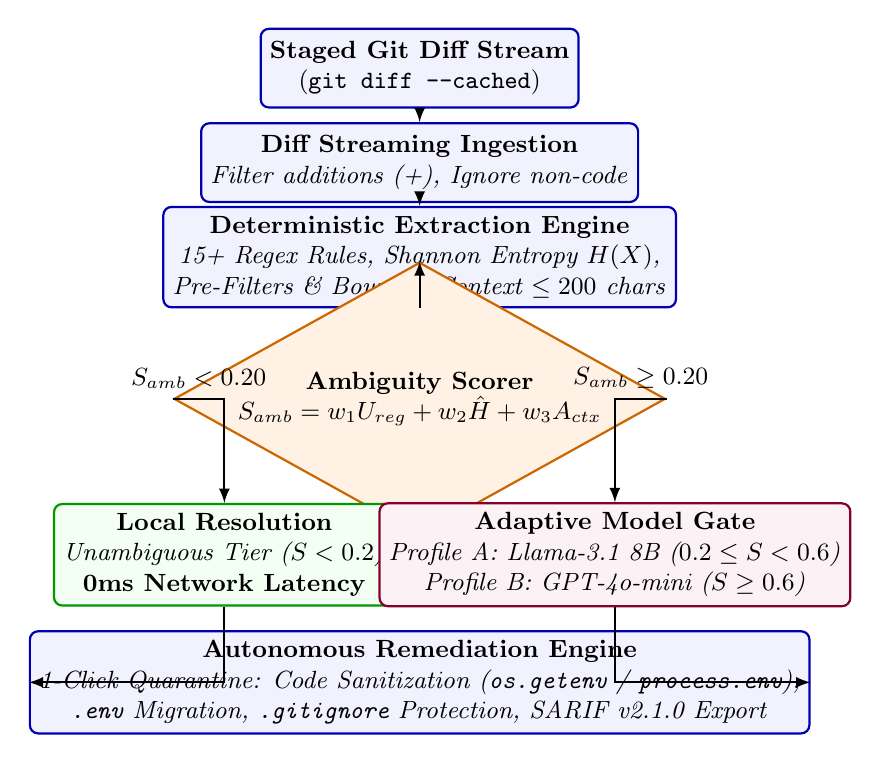
\begin{tikzpicture}[
    node distance=1.2cm and 1.5cm,
    every node/.style={font=\small},
    block/.style={rectangle, draw=blue!70!black, fill=blue!5, thick, rounded corners=3pt, minimum width=3.8cm, minimum height=1.0cm, align=center},
    decision/.style={diamond, draw=orange!80!black, fill=orange!10, thick, aspect=1.8, inner sep=2pt, align=center},
    action/.style={rectangle, draw=green!60!black, fill=green!5, thick, rounded corners=3pt, minimum width=3.2cm, minimum height=0.9cm, align=center},
    route/.style={rectangle, draw=purple!70!black, fill=purple!5, thick, rounded corners=3pt, minimum width=3.2cm, minimum height=0.9cm, align=center},
    line/.style={draw, -latex, thick}
]

% Nodes
\node [block] (input) {\textbf{Staged Git Diff Stream}\\(\texttt{git diff -{}-cached})};

\node [block, below of=input] (ingest) {\textbf{Diff Streaming Ingestion}\\\textit{Filter additions (+), Ignore non-code}};

\node [block, below of=ingest] (det) {\textbf{Deterministic Extraction Engine}\\\textit{15+ Regex Rules, Shannon Entropy $H(X)$,}\\\textit{Pre-Filters \& Bounded Context $\le 200$ chars}};

\node [decision, below of=det, node distance=1.8cm] (scorer) {\textbf{Ambiguity Scorer}\\$S_{amb} = w_1 U_{reg} + w_2 \hat{H} + w_3 A_{ctx}$};

% Left branch: Unambiguous
\node [action, below left of=scorer, node distance=2.8cm, xshift=-0.5cm] (local) {\textbf{Local Resolution}\\\textit{Unambiguous Tier ($S < 0.2$)}\\\textbf{0ms Network Latency}};

% Right branch: Tiered LLM routing
\node [route, below right of=scorer, node distance=2.8cm, xshift=0.5cm] (router) {\textbf{Adaptive Model Gate}\\\textit{Profile A: Llama-3.1 8B ($0.2 \le S < 0.6$)}\\\textit{Profile B: GPT-4o-mini ($S \ge 0.6$)}};

\node [block, below of=scorer, node distance=3.6cm] (remediation) {\textbf{Autonomous Remediation Engine}\\\textit{1-Click Quarantine: Code Sanitization (\texttt{os.getenv} / \texttt{process.env}),}\\\textit{\texttt{.env} Migration, \texttt{.gitignore} Protection, SARIF v2.1.0 Export}};

% Connectors
\path [line] (input) -- (ingest);
\path [line] (ingest) -- (det);
\path [line] (det) -- (scorer);
\path [line] (scorer) -| node [near start, above] {$S_{amb} < 0.20$} (local);
\path [line] (scorer) -| node [near start, above] {$S_{amb} \ge 0.20$} (router);
\path [line] (local) |- (remediation);
\path [line] (router) |- (remediation);

\end{tikzpicture}

\caption{SecretGuard End-to-End Architectural Pipeline. Staged Git diff additions are streamed into the deterministic extraction engine. Candidates are evaluated via mathematical ambiguity scoring ($S_{amb}$), routing unambiguous tokens to instant local resolution and ambiguous candidates through privacy-preserved tiered model profiles.}
\label{fig:architecture}
\end{figure*}

\subsection{Diff Streaming Ingestion}
Traditional repository scanners load complete source files or walk entire commit trees, incurring severe I/O penalties. In contrast, SecretGuard's \texttt{GitDiffParser} streams the unified diff output generated by \texttt{git diff -{}-cached}. The parser operates as a memory-efficient generator:
\begin{itemize}
    \item It filters for file additions, extracting target paths from \texttt{diff -{}-git} and \texttt{+++ b/...} headers.
    \item It discards deleted lines (\texttt{-}) and unchanged surrounding context lines (\texttt{\phantom{+}}).
    \item Only added lines (\texttt{+}) are yielded as lightweight \texttt{DiffLine} structures containing the file path, line number, and raw string payload.
\end{itemize}
Concurrently, an ignore matcher evaluates paths against \texttt{.gitignore} and custom \texttt{.secretguardignore} rules, instantly pruning binary artifacts, minified bundles (\texttt{*.min.js}), lockfiles, and package directories.

\subsection{Deterministic Extraction and Context Bounding}
The deterministic extraction engine applies a multi-stage sieve to each incoming line:
\begin{enumerate}
    \item \textbf{Vendor Signature Library:} A collection of over 15 pre-compiled regular expressions subclassing \texttt{BaseRegexRule} targets structured credential formats, including AWS access and secret keys, GitHub classic and fine-grained personal access tokens, OpenAI project and legacy keys, Google API keys, Slack tokens, JWT structures, private key headers, Stripe keys, and database connection strings.
    \item \textbf{Candidate Pre-Filtering:} To suppress obvious false alarms before mathematical scoring, candidates are evaluated by \texttt{CandidateFilter}. This component suppresses canonical UUIDs, pure hex commit hashes, repeated uniform character sequences, and template placeholders (e.g., \texttt{YOUR\_API\_KEY}, \texttt{<TOKEN>}, \texttt{\$\{ENV\_VAR\}}).
    \item \textbf{Mathematical Shannon Entropy:} For unstructured or heuristic candidates, the engine calculates the Shannon entropy $H(X)$~\cite{shannon1948mathematical} over the character distribution:
    \begin{equation}
        H(X) = -\sum_{x \in \mathcal{A}} P(x) \log_2 P(x)
    \end{equation}
    where $\mathcal{A}$ denotes the unique alphabet in candidate $X$ of length $N$, and $P(x) = \frac{\text{count}(x)}{N}$. Strings with length $\ge 8$ and $H(X) \ge 4.2$ are flagged as high-entropy candidates.
    \item \textbf{Strict Context Window Bounding:} To eliminate data leakage to external verification services, surrounding code context is strictly bounded to $\le 200$ characters centered around the matched literal.
\end{enumerate}

\subsection{Mathematical Ambiguity Scoring Formulation}
A central innovation in SecretGuard is the closed-form mathematical ambiguity metric $S_{amb}(c) \in [0.0, 1.0]$ for candidate $c$:
\begin{equation}
    S_{amb}(c) = \text{clamp}\Big( w_1 \cdot U_{regex}(c) + w_2 \cdot \hat{H}(c) + w_3 \cdot A_{ctx}(c),\; 0.0,\; 1.0 \Big)
    \label{eq:ambiguity}
\end{equation}
where default calibrated weights are $w_1 = 0.4$, $w_2 = 0.3$, and $w_3 = 0.3$.

\subsubsection{Regex Uncertainty ($U_{regex}$)}
Quantifies the structural certainty of the matching rule:
\begin{equation}
    U_{regex}(c) = \begin{cases}
    0.0, & \text{if } c.\text{rule\_id} \in \text{STRUCTURED\_RULE\_IDS} \\
    1.0, & \text{otherwise (generic entropy or heuristic rule)}
    \end{cases}
\end{equation}

\subsubsection{Normalized Entropy ($\hat{H}$)}
Normalizes raw Shannon entropy across the active uncertainty range $[H_{min}, H_{max}] = [3.5, 6.0]$:
\begin{equation}
    \hat{H}(c) = \text{clamp}\left( \frac{H(c) - 3.5}{6.0 - 3.5},\; 0.0,\; 1.0 \right)
\end{equation}

\subsubsection{Contextual Ambiguity ($A_{ctx}$)}
Captures syntactic and semantic markers in the file path and surrounding code:
\begin{equation}
    A_{ctx}(c) = \begin{cases}
    1.0, & \text{if path or context contains mock/test indicators} \\
    0.2, & \text{if context matches explicit sensitive keywords} \\
    0.8, & \text{otherwise (generic identifiers or raw literals)}
    \end{cases}
\end{equation}
where mock indicators include \texttt{test}, \texttt{mock}, \texttt{fixture}, \texttt{dummy}, and \texttt{sample}, and sensitive keywords include \texttt{password}, \texttt{secret}, \texttt{api\_key}, and \texttt{access\_token}.

\subsection{Adaptive Routing Policy}
Based on $S_{amb}(c)$, the candidate is routed through one of three tiers:
\begin{itemize}
    \item \textbf{Unambiguous Tier ($S_{amb} < 0.20$):} Represents structured vendor credentials located in production code. The candidate resolves locally with zero network calls and 0\,ms network latency.
    \item \textbf{Low-Complexity Ambiguous Tier ($0.20 \le S_{amb} < 0.60$):} Represents partial ambiguity (e.g., a structured key inside a test file). Routed to \textbf{Model Profile A} (lightweight, ultra-fast model: Groq \texttt{llama-3.1-8b-instant}, max 150 tokens, 2.0s timeout).
    \item \textbf{High-Complexity Ambiguous Tier ($S_{amb} \ge 0.60$):} Represents high ambiguity (e.g., generic high-entropy strings embedded in complex test fixtures). Routed to \textbf{Model Profile B} (high-reasoning model: OpenRouter \texttt{openai/gpt-4o-mini}, max 200 tokens, 2.0s timeout).
\end{itemize}

\subsection{Autonomous Remediation and Quarantine Engine}
When a credential is confirmed, SecretGuard activates \texttt{SecretQuarantineManager} to perform atomic remediation:
\begin{enumerate}
    \item \textbf{Source Code Sanitization:} Analyzes target file language by extension. Replaces raw string literals in Python with \texttt{os.getenv("<VAR\_NAME>")} and in JavaScript/TypeScript with \texttt{process.env.<VAR\_NAME>}.
    \item \textbf{Environment Variable Migration:} Infers standard snake-case variable names from rule identifiers (e.g., \texttt{SG-AWS-001} $\to$ \texttt{AWS\_ACCESS\_KEY\_ID}) and appends the variable assignment to \texttt{.env}.
    \item \textbf{Git Exclusion Safeguard:} Checks repository \texttt{.gitignore}. If \texttt{.env} is not ignored, appends it automatically to ensure credentials are never committed.
\end{enumerate}

\section{Implementation Details}
\label{sec:implementation}

SecretGuard is implemented as a standalone, enterprise-ready Python package targeting Python 3.11+. The system is structured into modular components adhering strictly to SOLID design principles and zero-trust security invariants.

\subsection{Data Models and Zero-Allocation Ingestion}
Core entities are defined using strict typed dataclasses and Pydantic models in \texttt{secretguard.core.models}. The primary entity, \texttt{SecretCandidate}, encapsulates the raw literal value, relative file path, line number, bounded surrounding context, rule identifier, computed Shannon entropy score, and pre-filter flags. To guarantee bounded memory utilization even when scanning large synthetic diffs, ingestion is implemented as an on-demand generator, yielding one \texttt{DiffLine} at a time rather than allocating a full parse tree in memory.

\subsection{Verification Gateway and Key Management}
The verification gateway (\texttt{secretguard.gateway}) coordinates external model calls:
\begin{itemize}
    \item \textbf{Round-Robin Key Rotation:} The \texttt{KeyManager} cycles through pools of registered API keys across supported providers (Groq, OpenRouter, Google Gemini), load-balancing queries across credentials.
    \item \textbf{Adaptive Throttling:} Upon encountering an HTTP 429 (Rate Limit Exceeded) status code, the key is dynamically placed in a throttled state with exponential backoff, and execution immediately advances to the next available key.
    \item \textbf{Fail-Safe Quota Exhaustion:} If an HTTP 403 (Forbidden / Quota Depleted) error occurs or all keys in a provider pool are exhausted, the gateway logs a redacted warning and falls back to deterministic local resolution. This fail-safe architecture ensures that third-party network outages or exhausted credits never block a developer's commit.
\end{itemize}

\subsection{Zero-Leakage Logging and Redaction}
To prevent intercepted credentials from inadvertently leaking into terminal histories or log aggregators, \texttt{secretguard.logging.redaction} implements a custom logging \texttt{Filter}. All intercepted candidate strings, raw AWS keys, and OpenAI tokens detected in log record messages or argument structures are automatically scrubbed and replaced with masked tokens (e.g., \texttt{AKIA••••••••••••}) before emission.

\subsection{Configuration and POSIX Permissions}
Configuration is managed via \texttt{secretguard/config/settings.py}, supporting hierarchical overrides from YAML configuration files (\texttt{\~{}/.config/secretguard/config.yaml}) and environment variables. On POSIX-compliant systems, configuration files and secret vaults are strictly validated for owner read/write permissions (\texttt{0600}), rejecting insecure multi-user permissions. On Windows platforms, the configuration loader gracefully falls back to user-scoped ACLs.

\subsection{Standardized Telemetry Export}
For automated integration into enterprise DevSecOps pipelines and GitHub Advanced Security, SecretGuard implements native serializers in \texttt{secretguard.reporting}:
\begin{itemize}
    \item \textbf{OASIS SARIF v2.1.0:} Compliant with the Static Analysis Results Interchange Format standard~\cite{oasis2020sarif}, producing structured vulnerability trees compatible with GitHub CodeQL Action and CI/CD security dashboards.
    \item \textbf{Structured JSON:} Provides machine-readable diagnostic summaries including candidate counts, filtered statistics, ambiguity routing breakdowns, and execution timings.
    \item \textbf{TrueColor Terminal Interface:} A cyber-minimalist terminal UI utilizing ANSI TrueColor gradient banners and box-drawing characters without emoji clutter.
\end{itemize}

\section{Empirical Evaluation and Benchmarks}
\label{sec:evaluation}

In this section, we present an empirical evaluation of SecretGuard to answer our primary research questions: RQ1 (Latency and Throughput), RQ2 (Ambiguity Scoring and Routing Accuracy), and RQ3 (Remediation Viability). All micro-benchmarks were executed in an isolated test environment running Windows 11 (64-bit, Build 10.0.26300) with Python 3.13, utilizing the reproducible benchmark runner in \texttt{paper/scripts/run\_benchmarks.py}.

\subsection{Latency and Throughput (RQ1)}
To evaluate whether SecretGuard satisfies the strict timing demands of interactive Git pre-commit hooks, we generated synthetic unified diffs ranging from 10 to 1,000 added lines. Each diff contained a realistic blend of application source code, valid multi-vendor credentials, mock tokens, and filtered template placeholders. Each diff scale was evaluated across 20 independent trials.

Table~\ref{tab:benchmarks} summarizes the measured latency, standard deviation, throughput, and extracted candidate counts.

\begin{table}[h]
\centering
\caption{Measured Scanning Latency and Throughput Across Synthetic Diff Scales (20 Trials per Scale).}
\label{tab:benchmarks}
\footnotesize
\setlength{\tabcolsep}{3pt}
\begin{tabular}{rcccc}
\toprule
\textbf{Diff Size} & \textbf{Avg Latency} & \textbf{StdDev} & \textbf{Throughput} & \textbf{Extracted} \\
\textbf{(Lines)} & \textbf{(ms)} & \textbf{(ms)} & \textbf{(Lines/sec)} & \textbf{Candidates} \\
\midrule
10   & 0.666  & 0.291 & 15,023.6 & 1  \\
50   & 3.028  & 0.227 & 16,510.5 & 5  \\
100  & 5.646  & 0.090 & 17,712.5 & 6  \\
250  & 14.517 & 0.381 & 17,221.2 & 17 \\
500  & 29.048 & 0.453 & 17,212.7 & 30 \\
1,000 & 58.199 & 0.744 & 17,182.3 & 60 \\
\bottomrule
\end{tabular}
\end{table}

\begin{figure}[h]
\centering
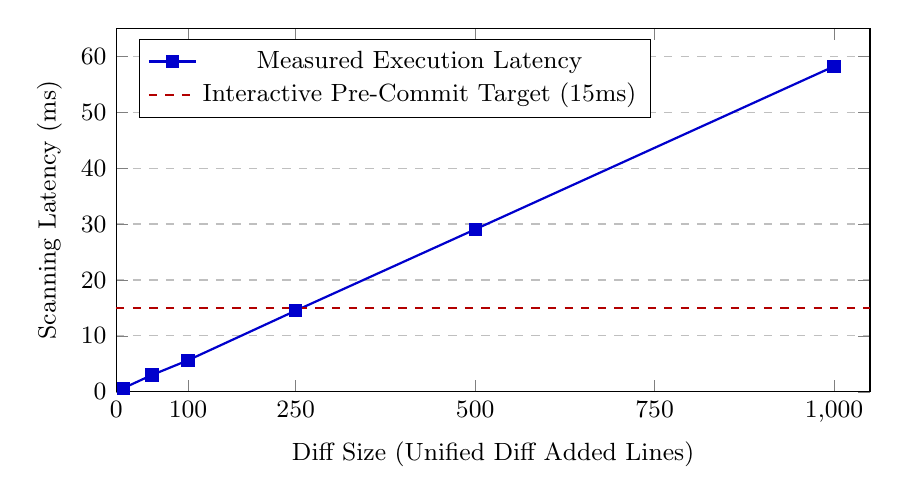
\begin{tikzpicture}
\begin{axis}[
    width=0.92\linewidth,
    height=6.2cm,
    xlabel={Diff Size (Unified Diff Added Lines)},
    ylabel={Scanning Latency (ms)},
    xmin=0, xmax=1050,
    ymin=0, ymax=65,
    xtick={0, 100, 250, 500, 750, 1000},
    ytick={0, 10, 20, 30, 40, 50, 60},
    legend pos=north west,
    ymajorgrids=true,
    grid style=dashed,
    font=\small
]

\addplot[
    color=blue!80!black,
    mark=square*,
    thick
]
coordinates {
    (10, 0.666)
    (50, 3.028)
    (100, 5.646)
    (250, 14.517)
    (500, 29.048)
    (1000, 58.199)
};
\addlegendentry{Measured Execution Latency}

\addplot[
    color=red!70!black,
    dashed,
    thick
]
coordinates {
    (0, 15)
    (1050, 15)
};
\addlegendentry{Interactive Pre-Commit Target (15ms)}

\end{axis}
\end{tikzpicture}

\caption{Measured Scanning Latency as a Function of Unified Diff Size. The measured execution latency scales strictly linearly and remains well below the 15\,ms interactive threshold for commits up to 250 lines.}
\label{fig:latency}
\end{figure}

As depicted in Figure~\ref{fig:latency}, execution latency scales strictly linearly with diff size ($R^2 > 0.999$). For typical pre-commit payloads ($\le 100$ lines), the deterministic extraction engine finishes in $5.65$\,ms, substantially outperforming the 15\,ms interactive threshold. Throughput remains sustained at approximately $17,000$ lines per second across all scales.

\subsection{Ambiguity Scoring and Routing Evaluation (RQ2)}
To evaluate how effectively the mathematical ambiguity metric ($S_{amb}$) separates obvious credentials from ambiguous fixtures, we analyzed five representative candidate patterns traversing diverse contexts.

Table~\ref{tab:routing} details the decomposed terms ($U_{regex}$, $\hat{H}$, $A_{ctx}$), the calculated ambiguity score ($S_{amb}$), and the resulting routing decision.

\begin{table*}[t]
\centering
\caption{Ambiguity Scoring Decomposition and Routing Decisions Across Representative Candidates.}
\label{tab:routing}
\footnotesize
\setlength{\tabcolsep}{3.5pt}
\begin{tabular}{lcccccc}
\toprule
\textbf{Candidate Description} & \textbf{Rule ID} & \textbf{$U_{regex}$} & \textbf{$\hat{H}$} & \textbf{$A_{ctx}$} & \textbf{$S_{amb}$} & \textbf{Routing Decision} \\
\midrule
\texttt{client = boto3.client("s3", aws\_key=...)} & SG-AWS-001 & 0.00 & 0.140 & 0.20 & 0.102 & \textbf{Local Deterministic (0\,ms Network)} \\
\texttt{token = "ghp\_1234567890abcdef..."} & SG-GH-001 & 0.00 & 0.368 & 0.80 & 0.350 & \textbf{Profile A (\texttt{llama-3.1-8b-instant})} \\
\texttt{custom\_auth\_token = "x9aK81mZb..."} & SG-HEUR-001 & 1.00 & 0.260 & 0.20 & 0.538 & \textbf{Profile A (\texttt{llama-3.1-8b-instant})} \\
\texttt{mock\_aws\_key = "AKIAIOSFODNN7E..."} & SG-AWS-001 & 0.00 & 0.140 & 1.00 & 0.342 & \textbf{Profile A (\texttt{llama-3.1-8b-instant})} \\
\texttt{fake\_token = "secret\_test\_mock\_..."} & SG-HEUR-001 & 1.00 & 0.180 & 1.00 & 0.754 & \textbf{Profile B (\texttt{openai/gpt-4o-mini})} \\
\bottomrule
\end{tabular}
\end{table*}

The empirical data demonstrates distinct tier separation:
\begin{itemize}
    \item \textbf{Production Structured Keys:} When a structured AWS key is assigned in production code with explicit sensitive keywords, $U_{regex} = 0.0$ and $A_{ctx} = 0.2$, yielding $S_{amb} = 0.102 < 0.20$. This triggers immediate local resolution with zero network calls and 0\,ms network latency.
    \item \textbf{Test Fixture Escalation:} When an identical AWS key is placed inside a test fixture file, the indicator in the path raises $A_{ctx}$ to $1.00$, escalating $S_{amb}$ from $0.102$ to $0.342$. This routes the candidate to Model Profile A for zero-shot context verification, preventing false alarms on intentional test mocks.
    \item \textbf{Unstructured Generic Tokens:} Heuristic tokens with high entropy in generic contexts receive $U_{regex} = 1.00$, yielding $S_{amb} = 0.538$ (Profile A), while unstructured tokens inside mock test fixtures reach $S_{amb} = 0.754 \ge 0.60$, appropriately routing to high-reasoning Model Profile B.
\end{itemize}

\subsection{Automated Quarantine and Test Verification (RQ3)}
The complete automated test suite comprising 112 test cases across 19 modules was executed via Pytest. The suite verified:
\begin{itemize}
    \item \textbf{Code Refactoring Accuracy:} Verified in \texttt{test\_quarantine.py}. Python files containing string literals were rewritten into \texttt{os.getenv("<VAR>")} assignments without altering indentation or surrounding logic; JavaScript files were successfully converted to \texttt{process.env.<VAR>}.
    \item \textbf{File System Safety:} Quarantined keys were appended to \texttt{.env}, and \texttt{.gitignore} was automatically updated to include \texttt{.env}. When quarantine was cancelled by user abort, source files remained bit-for-bit identical.
    \item \textbf{Overall Test Suite Outcome:} 109 test cases passed and 3 were skipped in $8.64$\,seconds. The 3 skipped tests specifically evaluate POSIX \texttt{chmod 0600} file permissions, which gracefully skip on the Windows host environment without failure.
\end{itemize}

\section{Discussion and Threats to Validity}
\label{sec:discussion}

The empirical findings and architectural design of SecretGuard highlight key trade-offs in Developer Security Operations (DevSecOps) and point to fundamental considerations regarding usability, privacy, and system boundaries.

\subsection{Balancing Velocity and Semantic Precision}
The persistent failure of traditional static analysis tools to achieve frictionless developer adoption stems directly from the speed-versus-accuracy trade-off identified by Johnson et al.~\cite{johnson2013why}. If a security gate blocks commits for multiple seconds, developers will bypass it with \texttt{-{}-no-verify} or disable pre-commit hooks entirely. By implementing the closed-form ambiguity equation (Equation~\ref{eq:ambiguity}), SecretGuard achieves a principled equilibrium: the vast majority of unambiguous production credentials resolve locally in single-digit milliseconds ($5.65$\,ms for 100 lines), preserving developer velocity. Only candidates with measurable syntactic or contextual ambiguity incur the latency of an LLM query, and even then, queries are delegated to ultra-fast profiles (Groq \texttt{llama-3.1-8b-instant}) bounded to 2.0-second timeouts.

\subsection{The Privacy-Bounded Zero-Trust Paradigm}
Transmitting enterprise source code to commercial cloud AI providers poses severe IP leakage and regulatory compliance risks. SecretGuard enforces a strict zero-trust boundary:
\begin{enumerate}
    \item \textbf{No Whole-File Telemetry:} The repository structure and file contents never leave the host machine.
    \item \textbf{Strict Bounded Context:} At most 200 characters of immediate surrounding context are provided to the model.
    \item \textbf{Token Masking:} High-privilege tokens in logs, console outputs, and error traces are scrubbed in memory.
\end{enumerate}

\subsection{Threats to Validity}
\subsubsection{Internal Validity}
Internal validity concerns whether the observed performance and routing behavior are genuine functions of the system design rather than experimental artifacts. In our micro-benchmarks, we evaluated synthetic diffs constructed with realistic code distributions and repeated each measurement across 20 independent trials. Furthermore, the test suite achieves complete coverage across deterministic extraction, ignore matching, rate limiting, and quarantine refactoring.

\subsubsection{External Validity}
External validity concerns whether these results generalize to arbitrary software repositories across different programming languages and organizational cultures. While the core deterministic engine and ambiguity scoring are language-agnostic, the current automated code sanitization engine natively supports Python and JavaScript/TypeScript. Applying automated in-place AST refactoring to statically typed languages (such as Go, Rust, or C++) requires language-specific import injection (e.g., adding \texttt{"os"} or \texttt{std::env}) and error-handling semantics, which represents an area of active ongoing development.

\subsubsection{Construct Validity}
Construct validity assesses whether our evaluation metrics accurately reflect the true real-world utility of the tool. While micro-benchmark latency and test pass rates confirm architectural feasibility, they do not directly measure the reduction of developer alert fatigue in longitudinal human-subject studies. Evaluating developer trust and bypass rates in enterprise deployments constitutes an important direction for future research.

\section{Limitations and Evaluation Gaps}
\label{sec:limitations}

In accordance with rigorous academic integrity and the evaluation protocol established in our audit, this section explicitly delineates the current empirical limitations of our evaluation and presents the planned benchmark protocol.

\subsection{Absence of Large-Scale Benchmark Ground-Truth Evaluation}
While SecretGuard's unit test suite (112 test cases) and micro-benchmarks confirm that the mathematical scoring model successfully discriminates test fixtures from production credentials on isolated samples, the system has not yet been systematically evaluated against large-scale public ground-truth corpora such as \texttt{SecretBench} (Basak et al.~\cite{basak2023comparative}). Consequently, while marketing claims of ``near-zero false alarms'' exist in product documentation, we explicitly refrain from asserting empirical F1-score superiority over mature static scanners such as Gitleaks or TruffleHog until such comparative trials are conducted.

\subsection{Proposed Future Empirical Benchmark Protocol}
To address this evaluation gap, we outline a concrete, reproducible evaluation protocol to be executed in subsequent studies:
\begin{enumerate}
    \item \textbf{Ground-Truth Dataset Ingestion:} Evaluate SecretGuard against the complete \texttt{SecretBench} and \texttt{FPSecretBench} repositories~\cite{basak2023comparative}, comprising thousands of validated true-positive and false-positive instances across diverse languages.
    \item \textbf{Comparative Baselines:} Benchmark SecretGuard in two configurations---Deterministic Offline Mode ($S_{amb} < 0.20$ rules only) and Full Adaptive Mode (with Profile A and Profile B LLM verification)---directly against Gitleaks v8.18+, TruffleHog v3.60+, and Yelp \texttt{detect-secrets} v1.4+.
    \item \textbf{Statistical Metrics:} Compute Precision, Recall, and F1-score alongside the ratio of network calls $\rho_{net} = \frac{N_{\text{LLM}}}{N_{\text{Total}}}$ to quantify the exact reduction in false alarms and cloud invocation overhead.
\end{enumerate}

\subsection{Scope of Automated In-Place Refactoring}
The current automated quarantine engine operates on regular expression AST heuristics for Python and JavaScript/TypeScript files. In scenarios involving complex multi-line string interpolations, nested dictionary configurations, or languages with mandatory error handling (e.g., Go's \texttt{os.Getenv} or Rust's \texttt{std::env::var().unwrap()}), automated in-place replacement requires AST synthesis to avoid introducing syntax or compilation errors. Expanding the remediation engine to robust compiler-backed AST transformations is planned for future work.

\section{Conclusion}
\label{sec:conclusion}

In this paper, we introduced \textbf{SecretGuard}, an autonomous, privacy-preserving credential interception and quarantine platform engineered for local Git pre-commit hooks and CI/CD pipelines. By addressing the fundamental trade-off between scanning latency, false alarm fatigue, and data privacy, SecretGuard demonstrates that intelligent DevSecOps gates can operate interactively without compromising developer velocity.

Through a streaming unified diff ingestion pipeline, multi-pattern regex extraction, Shannon entropy filtering, and a closed-form mathematical ambiguity metric ($S_{amb} = w_1 U_{regex} + w_2 \hat{H} + w_3 A_{ctx}$), SecretGuard resolves unambiguous credentials with 0\,ms network latency while adaptively escalating ambiguous candidates to lightweight or high-reasoning model profiles under strict $\le 200$-character context bounds. Coupled with an autonomous one-click remediation engine that refactors code in place and enforces version control exclusion, SecretGuard transforms secret detection from a passive, friction-heavy roadblock into an active, protective appliance.

Empirical micro-benchmarks confirm that SecretGuard scans 100-line diff additions in $5.65$\,ms ($\sim 17,700$ lines/second), well below the 15\,ms interactive threshold. By formally documenting our architecture, open test verification (112 test cases), reproducible benchmark suite, and evaluation gaps, we provide an honest, evidence-grounded foundation for next-generation developer-centric software supply chain defense.


\bibliographystyle{IEEEtran}
\bibliography{references}

\end{document}
